\section{Convolution performance}
    We implemented two versions of the convolution algorithm as described before, the naïve version and the FFT version \ref{code:dqop}. We compared their performance when performing convolution on two $\Delta$Qs of equal bins. In theory, we should observe the naïve version delay quickly grow, while the FFT version have a log-linear growth. We observe the result in \cref{fig:conv_perf}.
    As expected, the naïve version has a time complexity of $\mathcal{O}(N^2)$ and quickly scales with the number of bins. This is clearly inefficient, as a more precise $\Delta$Q will result in a much slower program.

As for the FFT algorithm, it is slightly slower when the number of bins is lower than 100. This is due to the FFTW3 routine having slightly higher overhead. Moreover, if we look closer at the FFT graph, we can observe slight increases after we surpass powers of 2 (e.g. at 600 $>$ 512, 300 $>$ 256 \dots). This is because the algorithm is based on $\Delta$Qs which are zero-padded to the nearest power of 2, to make the calculation faster.

While we limit the number of bins to 1000 right now, this limit could potentially be increased as the FFT convolution algorithm is very efficient (0.5 ms for 1024 bins).

    \begin{figure}[H]
        \begin{center}
            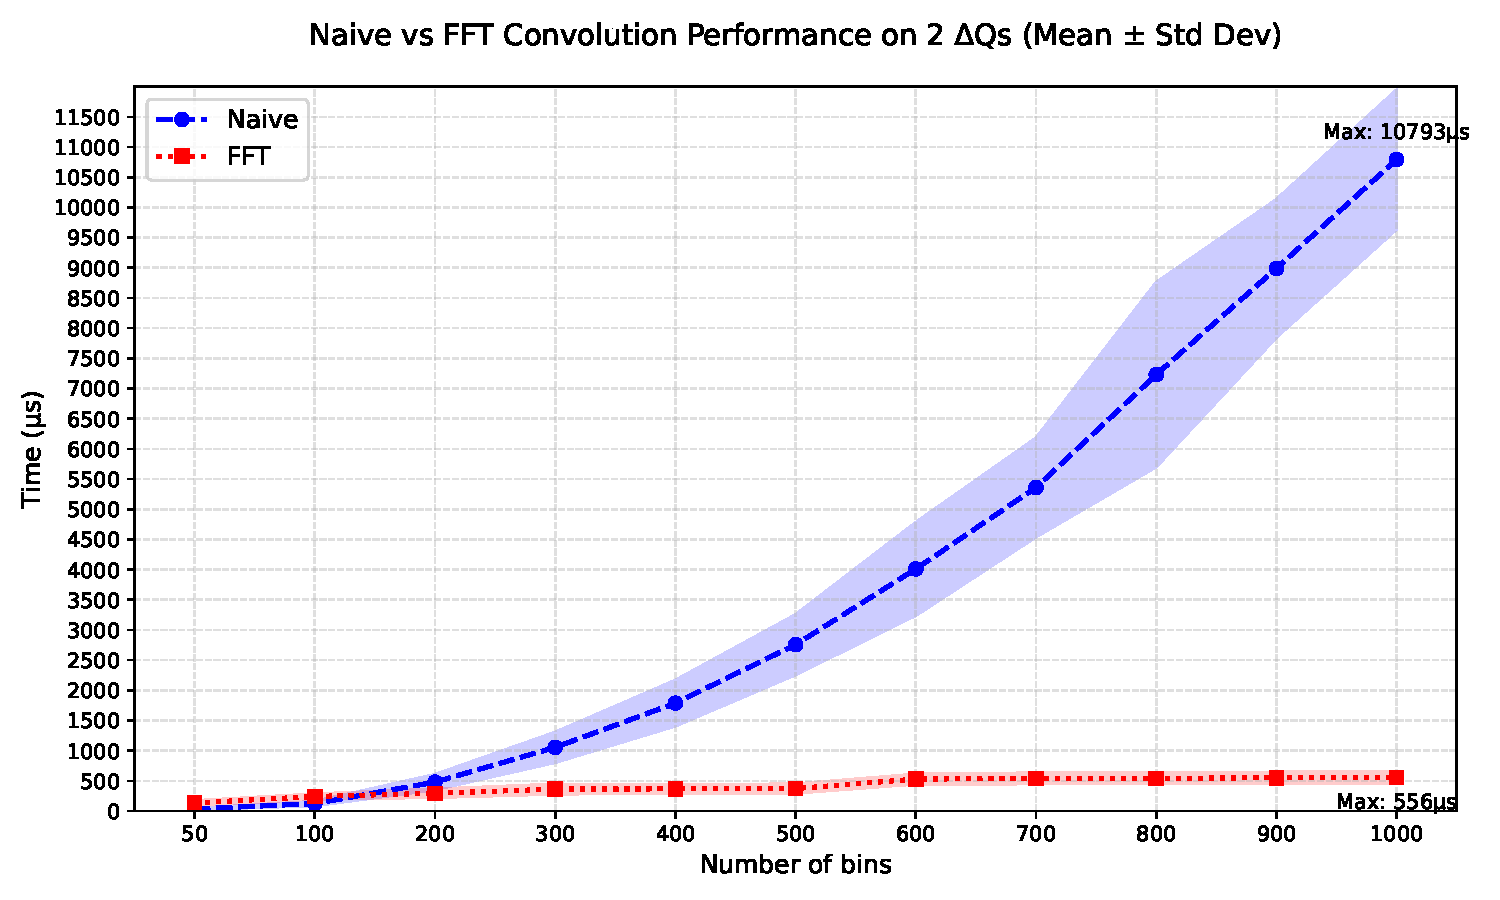
\includegraphics[width=0.85\textwidth]{img/conv_perf.pdf}
        \end{center}
        \caption{Performance comparison of FFT convolution and naïve convolution algorithms.}
        \label{fig:conv_perf}
    \end{figure}


